\documentclass{article}

% if you need to pass options to natbib, use, e.g.:
% \PassOptionsToPackage{numbers, compress}{natbib}
% before loading rl_project.

% to compile a camera-ready version, add the [final] option, e.g.:
 \usepackage[final]{rl_project}

% to avoid loading the natbib package, add option nonatbib:
% \usepackage[nonatbib]{rl_project}

\usepackage[utf8]{inputenc} % allow utf-8 input
\usepackage[T1]{fontenc}    % use 8-bit T1 fonts
\usepackage{hyperref}       % hyperlinks
\usepackage{url}            % simple URL typesetting
\usepackage{booktabs}       % professional-quality tables
\usepackage{amsfonts}       % blackboard math symbols
\usepackage{nicefrac}       % compact symbols for 1/2, etc.
\usepackage{microtype}      % microtypography
\usepackage{graphicx}
\usepackage{amsmath}
\usepackage{float}
\bibliographystyle{bathx}  

% Give your project report an appropriate title!

\title{Comparing a Range of Reinforcement Learning Algorithms to Solve a Classic Rocket Trajectory Problem}


% The \author macro works with any number of authors. There are two
% commands used to separate the names and addresses of multiple
% authors: \And and \AND.
%
% Using \And between authors leaves it to LaTeX to determine where to
% break the lines. Using \AND forces a line break at that point. So,
% if LaTeX puts 3 of 4 authors names on the first line, and the last
% on the second line, try using \AND instead of \And before the third
% author name.

\author{
  Alireza Samar, Arnold Gomes, Danny Demarco, Joseph Dowling, Robert Williams, Tyler Christie
  \\
  Department of Computer Science\\
  University of Bath\\
  Bath, BA2 7AY \\
  \texttt{\{as4731, ag2342, dd480, jtd38, rdw41, tc905\}@bath.ac.uk} \\
  %% examples of more authors
  %% \And
  %% Coauthor \\
  %% Affiliation \\
  %% Address \\
  %% \texttt{email} \\
  %% \AND
  %% Coauthor \\
  %% Affiliation \\
  %% Address \\
  %% \texttt{email} \\
  %% \And
  %% Coauthor \\
  %% Affiliation \\
  %% Address \\
  %% \texttt{email} \\
  %% \And
  %% Coauthor \\
  %% Affiliation \\
  %% Address \\
  %% \texttt{email} \\
}

\begin{document}


\maketitle
\newpage
\tableofcontents
\listoffigures
\newpage

\section{Problem Definition}
Application of reinforcement learning methods to modern artificial intelligence applications are both interesting and challenging, especially when the environment is unknown and there may be delayed rewards. This group project is an investigation into some of these methods and will attempt to train a number of agents to land a simulated spacecraft on the moon and compare their results for efficacy. To enable this the choice was made to make use of the LunarLander-v2 environment provided by OpenAI in their Gym package. The environment provides a classic rocket trajectory problem in which the rocket, starting at an elevated position is tasked with landing safely on a designated landing pad. There are two options in using this environment, discrete or continuous and we have chosen to use the discrete option. The 2d environment consists of the moon on the lower boundary with a section of it designated as the landing pad limited by the area between 2 flags, and an area of space above it in which the rocket may fly. The rocket itself is fitted with 2 legs to its base and three engines to provide thrust vertically or horizontally. To understand how the environment functions in more depth we can break it down into 4 main sections:


\begin{enumerate}
  \item States
  \begin{enumerate}
    \item Starting state\\
    Each episode begins with the rocket in the same position; at the top, center of the viewport. The variable factor is that there is a random force applied to the rockets center of mass at the outset.
    
    \item Observation space\\
     During an episode there are 8 possible states for the rocket to be in and consist of an 'x' and 'y' coordinate to denote its position, the linear velocity in both 'x' and 'y', the current angle of the rocket, the angular velocity, and two boolean values that represent whether each leg of the rocket is in contact with the ground or not. The landing pad is designated with (0,0) for its 'x' and 'y' coordinates.
  \end{enumerate}
  \item Actions\\
    There are 4 discrete actions available at any point: no action, fire right engine (left orientation), fire left engine (right orientation), fire main engine (upward orientation). Fuel is considered infinite and there is no range of acceleration, engines are binary and either on or off.
  
  \item Rewards\\
  Agents are incentivised/decentivised with the following reward structure:\\
  \begin{enumerate}
    \item Positive Rewards\\
    The reward for succesfully moving from the starting state and coming to rest at the landing pad range between 100-140 points depending on the accuracy of the landing. Each leg that is in contact with the ground provides an extra 10 points to incentivise a level approach to the landing pad. Once an episode is succesfully solved, a reward of 200 points is awarded.
    \item Negative Rewards\\
    To incentivise the agent to land on the platform as quickly as possible, negative rewards are given for each use of any of the engines in each frame of an episode of -0.3. If the rocket crashes (touches the moon), it receives -100 points.
  \end{enumerate}

  \item Episodes\\
  Each episode starts in the given starting state and runs until the terminal state is activated. A terminal state is activated in any of the following instances:
  \begin{enumerate}
    \item The rocket moves outside of the viewport (moves too far left, right, or up)
    \item The rocket crashes into the moon (misses the landing platform and hits the lower boundary)
    \item A sleep state is reached, i.e. not in motion and not involved in a collision. This includes once the rocket has succesfully landed on the landing platform.
  \end{enumerate}
\end{enumerate}

With these particulars in mind we can see that our agent is incentivised to direct the rocket from its starting position, to the landing pad with the minimal amount of engine use (fuel) as possible, while keeping the rocket stabilised as much as possible so that its legs may both make contact with the landing pad simultaneously. Incentivisation is produced by a large positive reward for reaching its platform, with bonus points for landing there in an upright position, and negative rewards for moving too far off course or colliding with the moons surface.


\section{Background}
Reinforcement learning is a powerful tool for decision making under uncertainty. Previous work has been done in solving the lunar lander environment using different techniques. This section will briefly introduce MDPs, Bellman Equation, Policy Gradient Methods, and other methods and then describe their strengths and weaknesses in solving the lunar lander problem.

Markov-decision processes (MDPs) are a type of mathematical model used in decision analysis and operations research. MDPs are used to model decision making in situations where the outcomes of a decision are partly determined by chance and partly by the decision maker's actions. In an MDP, the decision-maker is represented by a "agent" who takes actions in a discrete set of possible states, and a random process determines the state of the world at any given time. The MDP framework allows us to calculate the expected value of any decision, given the agent's current state and the probabilities of different outcomes in each state \citep{sutton1999between}.

MDPs are also used to model problems in machine learning and control theory. In machine learning, MDPs can be used to model the problem of learning how to take actions that maximize a reward. In control theory, MDPs can be used to model the problem of controlling a system to maximize a particular criterion, such as the expected value of the reward.

A common approach for such a state and action pair is Q-learning. In this approach, a Q-table gets updated iteratively to maximize the reward of every given state. This approach is framed by the Bellman Equation:

\begin{equation} \label{Bellman Equation}
  Q^{\ast}(s,a)=\mathbb{E}_{s^{'}\sim\varepsilon}[r+\gamma{max_{a^{'}}Q^{*}(s^{'},a^{'})}|s,a]
\end{equation}

Another common approach to solving MDPs is dynamic programming. Dynamic programming is a technique for breaking down a problem into smaller subproblems, solving each subproblem, and then combining the solutions to the subproblems to solve the original problem. This approach can be used in RL because the agent can learn which actions lead to the best outcomes by solving smaller MDPs.

There are a few different ways to implement dynamic programming for RL problems. The most common approach is to use a table to store the solutions to the subproblems. The table can be updated as the agent learns which actions lead to the best outcomes \citep{lewis2009reinforcement}.

The current reward and discounted maximum future reward can be concluded as the optimal value for a given pair of action-state. Since the number of Q-values would be computed as finite, the typical approach to solving iteratively is to use dynamic programming:

\begin{equation}
  Q_{i+1}(s,a)=\mathbb{E}[r+\gamma{max_{a^{'}}Q_{i}(s^{'},a^{'})}|s,a],{}\lim_{i\rightarrow{\infty}}Q_{i}=Q^{\ast}
\end{equation}

On the other hand, the policy gradient algorithm works by estimating the gradient of the expected reward function concerning the policy and then adjusting the policy accordingly. 

One of the benefits of the policy gradient algorithm is that it is relatively easy to implement. Additionally, the algorithm can adapt to changes in the environment, allowing the agent to learn new tasks and strategies.

In contrast, while described approaches try to optimise the Bellman Equation, the policy gradient aims to maximise the return by converging toward its policy.

Finally, Vanilla Policy Gradient (VPG) trains a policy known as the on-policy way \citep{peters2006policy}, which is different and often less sample efficient than the off-policy way, such as Deep Q-Network (DQN) \citep{dqn}.

While the off-policy methods take advantage of experiences from previous policies, the policy gradient cannot reduce the bias by reusing experience in picking trajectories of prior policies. This difference describes why policy gradient requires significantly higher training episods to return average \citep{Gadgil2020}.

\section{Method}
It was decided that 3 algorithms would be implemented to train our agents so that the different approaches could be compared and contrasted for efficacy against this particular problem. The 3 algorithms selected were; REINFORCE, a traditional policy gradient method chosen as a baseline method, and the more modern DQN and PPO algorithms. To give a better understanding of our chosen method PPO, we will first introduce TRPO, as this is where this method is derived from. 

\subsection{TRPO}
Trust Region Policy Optimization (TRPO) \citep{pmlr-v37-schulman15} is a policy-gradient method for on-policy, online learning. It uses the concept of a 'Trust Region' in policy space, which permits the policy to move only within a specific 'trusted' bound per gradient ascent step. This mitigates the risk of an agent moving into a region of policy space from which it cannot recover from a sample collected under a poor policy. \\\newline
An advantage estimate is calculated using a sampled discounted return under a policy $\pi$, parameterised by $\theta$, from an episode rollout, and a noisy value function estimate from a function approximator. Importance sampling is used to calculate the policy gradient from the old policy with a different sample distribution, and as such achieves greater sample efficiency than vanilla policy gradient methods (which use current policy to compute gradient). The objective function and target for optimisation is:
\begin{gather}
    \max_\theta\; \hat{\mathbb{E}_t}\left[\frac{\pi_\theta(a_t | s_t)}{\pi_{\theta_{old}}(a_t | s_t)}\hat{A_t}\right]\\
\text{subject to } \hat{\mathbb{E}_t}\left[KL\left[\pi_{\theta_{old}}(\cdot | s_t),\pi_\theta(\cdot|s_t)\right]\right] \leq \delta
\end{gather}
Where $KL$ is Kullback-Leibler Divergence \citep{Joyce2011}, and $\delta$ our trust region bound. Whilst the specifics of KL-Divergence are outside the scope of this project, it is essentially a statistical measure of the distance between two probability distributions; the policy update is subject to the constraint that KL-Divergence between the new and old policy must not exceed some hyperparameter $\delta$ for a gradient step. TRPO naturally falls into an Actor-Critic type model, where the value estimation is performed by the critic and the actor encodes the policy distribution. 
\subsection{PPO}
Proximal Policy Optimization \citep{schulman2017proximal} is a simplification and improvement over TRPO. Problems with TRPO were perceived to be complexity of implementation, and tractability of computation with regards to the KL-Divergence bound, which is an expensive operation with second-order optimisation required. A simpler bound was found to be more effective:
\begin{equation} \label{ppoupdate}
      L^{CLIP}(\theta) =  \hat{\mathbb{E}_t}\left[min(r_t(\theta)\hat{A^t},clip(r_t(\theta),1-\epsilon,1+\epsilon)\hat{A^t})\right]
\end{equation}
Where $r_t(\theta)$ is identical to the probability ratio from TRPO ($\frac{\pi_\theta(a_t | s_t)}{\pi_{\theta_{old}}(a_t | s_t)}$). The clip function replaces the KL-Divergence constraint, which clips the policy probability ratio such that the change does not exceed some hyperparameter $\epsilon$, typically 0.2 \citep{schulman2017proximal}. In addition to this, PPO provides some non-trivial code-level optimisations which significantly improve performance over TRPO \citep{Engstrom2020Implementation}. \\\newline
PPO was chosen for the proposed domain as it is relatively simple to implement, provides relatively good sample efficiency over other policy gradient methods, and is not particularly sensitive to hyperparameters \citep{schulman2017proximal}.
\subsection{DQN}
DQN (Deep-Q Networks) \citep{dqn} were the first foray into combining traditional reinforcement learning methods, Q-Learning \citep{qlearning}, with deep neural networks. Revolutionary at the time, it allowed an agent to approximate the Q values of previously intractable large state/action spaces. Using these networks in place of the policy $\pi(s,a)$, or value $q(s,a)$ functions.\\\newline
They work by feeding in the observable information of the environment, then training the network parameters via gradient descent with the aim of minimising a chosen loss function, typically the Mean Squared Error. The algorithm functions similarly to function approximated Q-learning, however it also incorporates a Replay memory and a target network. A target network is employed to tackle the instability of the algorithm caused by the presence of off-policy learning, function approximation and bootstrapping simulataneously. This is know as the deadly triad \citep{deadlytriad}. DQN addresses this by using a two separate networks, learning is performed from the target network onto the local network, and then the target network is updated periodically which improves the stability of the learning. The Replay memory is used to store all transitions $(S_{t},A_{t},R_{t},S_{t+1})$ encountered in the environment, then periodically a batch is sampled from these stored transitions and used to perform an update on the local network parameters, defined as:
\begin{equation}
\begin{aligned}
    &\text{Set} y_{j} = 
    \begin{cases}
    r_{j} & \text{ for terminal } s_{t+1}\\    
    r_{j} + \gamma\text{max}_{a'}Q(s_{t+1},a'; \theta_{2}) & \text{ for non terminal } s_{t+1}
    \end{cases}\\
    &\text{Perform gradient descent on } \nabla_{\theta_{1}}L_{\delta}(y_{j},\hat{q}_{1}(S_{j},A_{j};\boldsymbol{\theta}_{1}))
\end{aligned}
\end{equation}
In which every $C$ steps the target network $\theta_{2}$ is updated to the local network $\theta_{1}$.\\\newline
DQN was chosen for its historical significance, as it has led to many further improvements in modern reinforcement learning, such as the direct descendant \citet{rainbow} an amalgamation of many individual improvements to DQN, which was state of the art for its time, or any other deep reinforcement learning method which have built of the work of \citet{dqn}. 
\subsection{REINFORCE}
The final method we chose for this environment was REINFORCE \citep{williams1992simple}. REINFORCE is a traditional policy gradient method, but there are conflicting opinions about how exactly it should be implemented, possibly because as \citet{williams1992simple} defines it is fairly vague. The update function for network parameters $\theta$ is defined as \citep{10.5555/3312046}:
\begin{equation}
\theta_{t+1} = \theta_{t} + \alpha G_t\frac{\Delta_\theta\pi(A_t| S_t, \theta_t)}{\pi(A_t| S_t, \theta_t)}
\end{equation}
Where $\alpha$ is a hyperparameter controlling learning rate, $G_t$ is our Monte-Carlo sampled discounted returns, and $A_t,S_t$ are sampled actions and states respectively from a trajectory collected under policy $\pi$. By exploiting the likelihood ratio trick \citep{silver2015}, we can rewrite this as:
\begin{equation}
  \theta_{t+1} = \theta_{t} + \alpha G_t\Delta_\theta \text{log} \pi(A_t | S_t, \theta_t)
\end{equation}
Notice that unlike PPO, this update method only takes into account current policy, and as such results in much lower sample efficiency. In many instances, due to the high variance of Monte-Carlo sampling methods, an arbitrary baseline $b(s)$ is subtracted from $G_t$ in the update. $b(s)$ does not vary with $a$ and as such reduces per-update variance. \\\newline
The conflict surrounding implementation details for REINFORCE is with regard to the frequency of updates. Some accounts \citep{10.5555/3312046} suggest updates to the network should be done at every timestep, Others \citep{silver2015} suggest updates on some time horizon $T$, and \citet{williams1992simple} suggests a number of update points, including per-episode (i.e. traditional Monte-Carlo) updates. We chose to implement REINFORCE with per-episode updates, and no baseline. \\\newline
Using REINFORCE as a baseline policy gradient method, we are able to compare the results of our more modern PPO and DQN algorithms.
\section{Results and Discussion}
Algorithms were coded in base PyTorch \citep{NEURIPS2019_9015}. Due to time constraints, Bayesian Optimization was not carried out to discover optimal hyperparameters. As a result, hyperparameters were sourced from the original papers, or by consulting other online implementations and heuristic search. We make no claim that the hyperparameters used in the below experiments are optimal. Algorithms were run 10 times, and the graphs below are the average of these runs. Linear interpolation was used to fit data points per run to the average run length. Full graphs for every run can be found in Appendix X. 
\subsection{PPO}
PPO solved the Lunar Lander environment in an average of 608 episodes with a standard deviation of 102.6:
\begin{figure}[H]
  \centering
  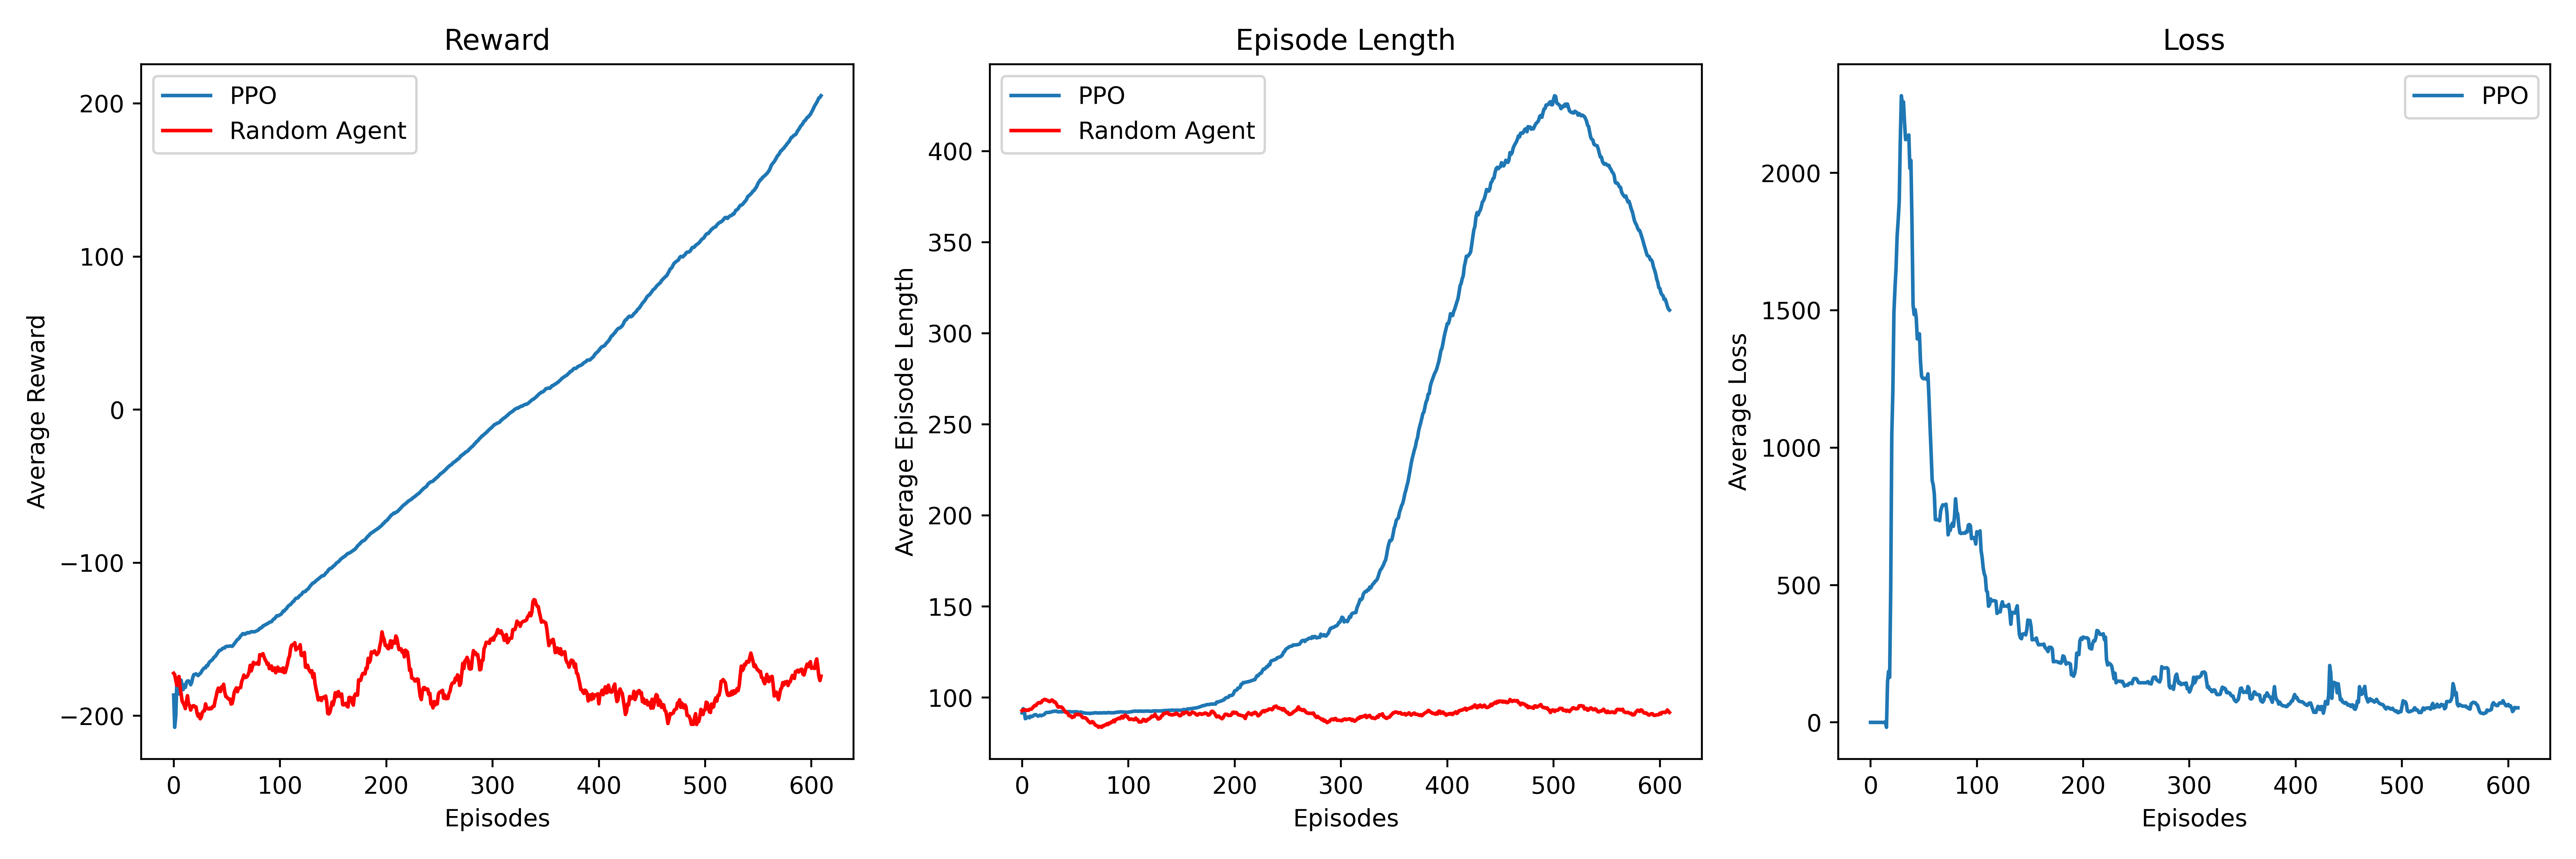
\includegraphics[scale=0.35]{1.png}
  \caption{(left-to-right) Average reward, episode length and loss for PPO.}
\end{figure}
\subsection{REINFORCE}
REINFORCE only solved this environment adequately in 3 out of 10 runs. Non-terminating runs were cut off after 5000 episodes:
\begin{figure}[H]
  \centering
  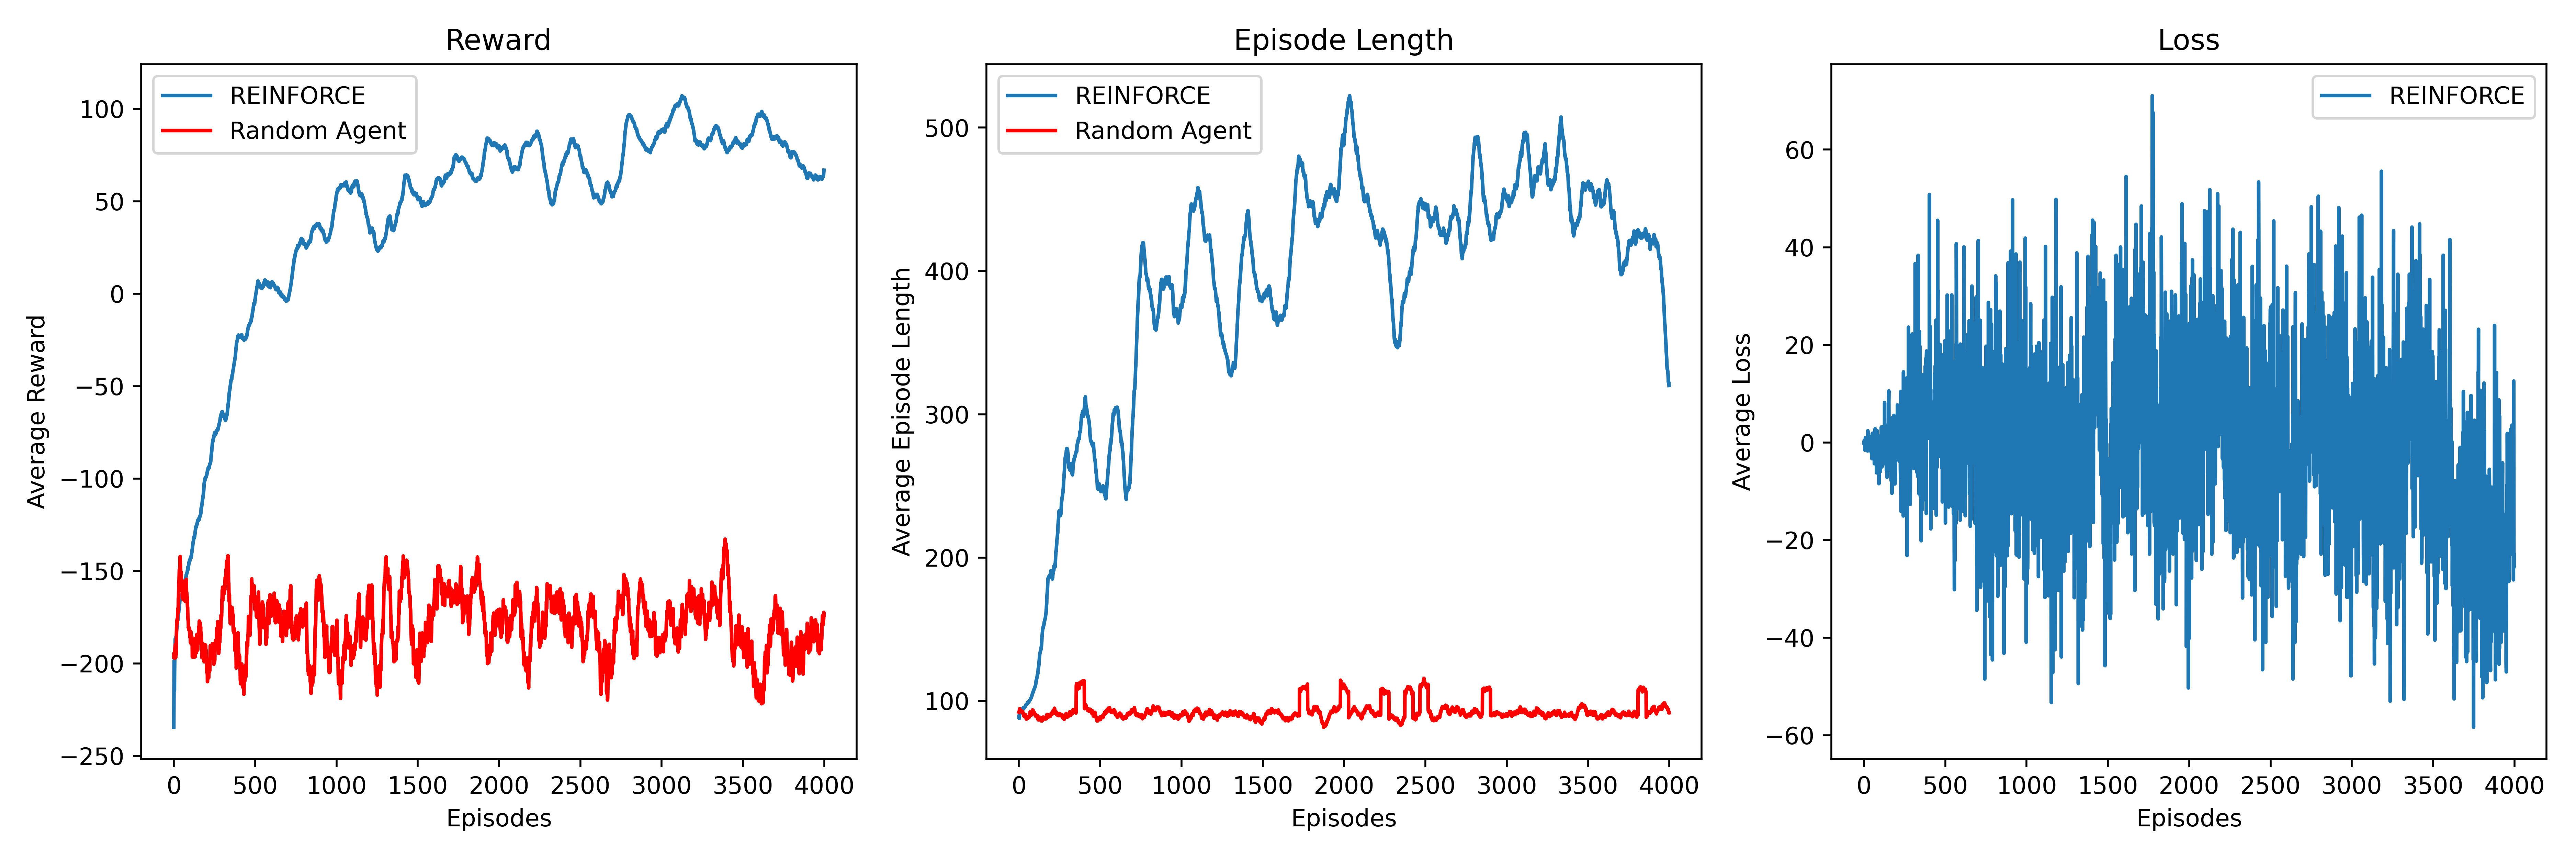
\includegraphics[scale=0.35]{2.png}
  \caption{(left-to-right) Average reward, episode length and loss for REINFORCE.}
\end{figure}
\subsection{DQN}
DQN solved the Lunar Lander environment in an average of 311 episodes with a standard deviation of 77.6:
\begin{figure}[H]
  \centering
  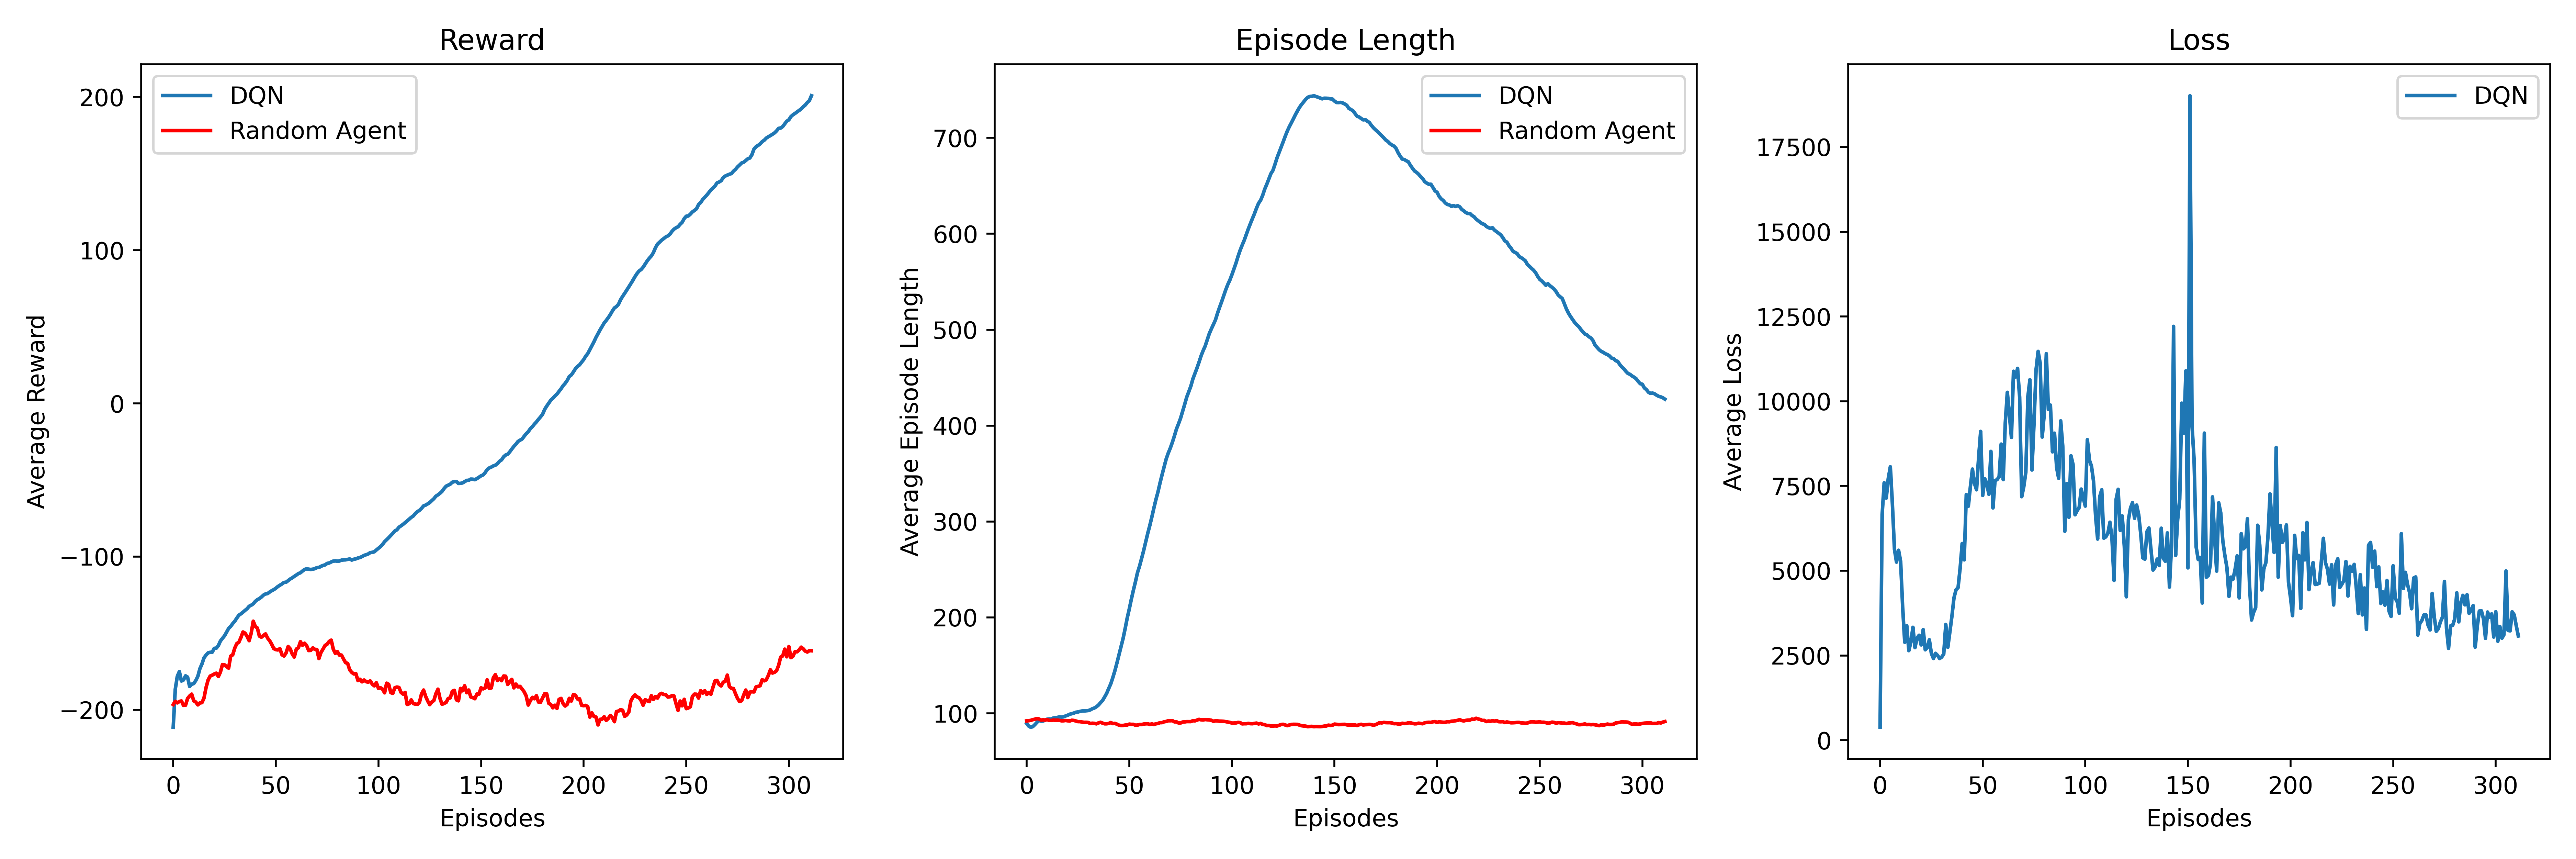
\includegraphics[scale=0.35]{3.png}
  \caption{(left-to-right) Average reward, episode length and loss for DQN.}
\end{figure}
\section{Future Work}
A discussion of potential future work you would complete if you had more
time.

The hyperparameters that have been used for each of the algorithms in this project may not be optimal, as has been previously mentioned. This is one area that could certainly be improved given more time. This could be done by applying a Bayesian Optimisation method, an approach that uses Bayes theorum to build a probibalistic model to optimise the objective function. This allows for selection of the hyperparemeters with the highest likelihood of effectiveness and can dramatically improve performance.

As DQN was introduced many years ago now, there has since been considerable work spent analysing and improving the algorithm. For future work we would seek to implement the much improved and much more complicated state of the art improvement, Rainbow \citep{rainbow}, an algorithm built from six individual improvements appended and combined with DQN. Work has been performed analysing Rainbow and found that it is a large improvement over base DQN in our chosen environment. Then additionally, among the included improvements, distributional RL \citep{distributionalrl} was the most necessary within this environment \cite{revisitingrainbow}. This is something we would like to examine and affirm in future work. 

\section{Personal Experience}
A discussion of your personal experience with the project, such as
difficulties or pleasant surprises you encountered while completing it.


\bibliography{references}

\newpage
\section*{Appendices}
If you have additional content that you would like to include in the appendices, please do so here.
There is no limit to the length of your appendices, but we are not obliged to read them in their entirety while marking. The main body of your report should contain all essential information, and content in the appendices should be clearly referenced where it's needed elsewhere.



Appendices should include (1) a detailed description of the problem domain,
including the states, actions, reward function, and transition dynamics; (2) all experimental
details so that the reader can fully replicate your experiments; and (3) how you selected your
hyperparameters (if applicable).
\subsection*{Appendix A: Example Appendix 1}
\subsection*{Appendix B: Example Appendix 2}

\end{document}

